\documentclass[11pt]{article}
\pagestyle{empty}
\setlength{\parindent}{0pt}
\usepackage[simplified]{pgf-umlcd}
\usepackage{pgf-umlsd}
\usepackage{tikz}

% \definecolor{umlfill1}{HTML}{f2e3c2}
% \definecolor{umltext1}{HTML}{020202}
% \definecolor{umldraw1}{HTML}{5c0505}


% \renewcommand {\umltextcolor}{umltext1}
% \renewcommand {\umlfillcolor}{umlfill1}
% \renewcommand {\umldrawcolor}{umldraw1}


\begin{document}
    
    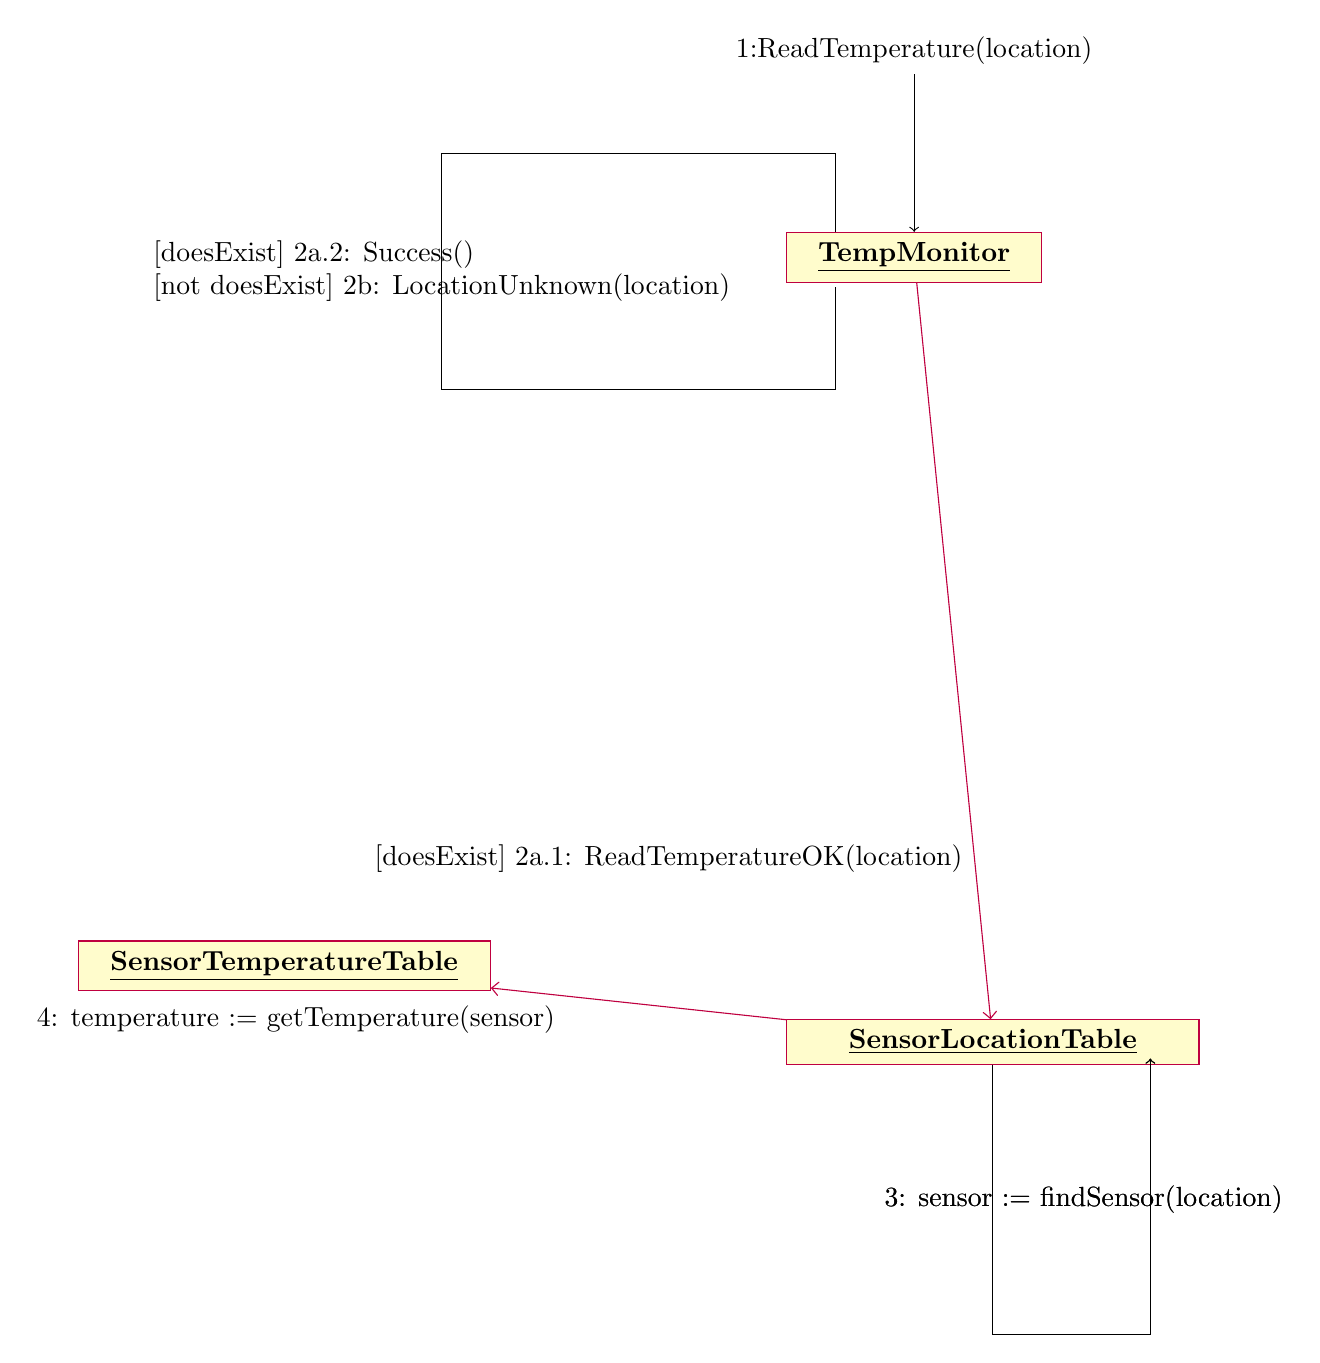
\begin{tikzpicture}
        
        
        \begin{object}[text width=3cm]{TempMonitor}{-3,6}
        \end{object}

        \begin{object}[text width=5cm]{SensorTemperatureTable}{-11,-3}
        \end{object}

        \begin{object}[text width=5cm]{SensorLocationTable}{-2,-4}
        \end{object}


        \draw[->] (-3,8) node[above] {1:ReadTemperature(location)} -- (TempMonitor);


        \draw[solid] (-4,6) -- (-4,7) -- (-9,7) -- (-9,4) node[midway, align=left] {[doesExist] 2a.2:  Success()\\ $$[not doesExist] 2b: LocationUnknown(location) } -- (-4,4) -- (-4,5.3);
        % \draw[solid] (TempMonitor) -- (0,-4);
        \unidirectionalAssociation{TempMonitor}{}{[doesExist] 
        2a.1: ReadTemperatureOK(location)}{SensorLocationTable}{}{}

        \unidirectionalAssociation{SensorLocationTable}{4: temperature := getTemperature(sensor)}{}{SensorTemperatureTable}{}{}
        
        \draw[->] (SensorLocationTable) -- (-2,-8) node[midway, right=-1.5cm] {3: sensor := findSensor(location)}-- (0,-8) -- (0,-4.5);

    
        \draw[->] (SensorLocationTable) -- (-2,-8) node[midway, right=-1.5cm] {3: sensor := findSensor(location)}-- (0,-8) -- (0,-4.5);
        

    
    \end{tikzpicture}

    % \begin{sequencediagram}
    % \newinst[6]{name}{Instance}
    % \end{sequencediagram}
\end{document}
